%! ~~~ Packages Setup ~~~ 
\documentclass[]{article}


% Math packages
\usepackage[usenames]{color}

% Deisgn
\usepackage{yfonts}
\usepackage{wrapfig}
\font\Cal=cmsy10 at 25pt
\textwidth=.5\textwidth
\def\pstart#1{\noindent\smash{\lower3ex\hbox{\llap{\Huge\frakfamily#1}}}
	\parshape=3 1.5em \dimexpr\hsize-1.5em 2em \dimexpr\hsize-2em 0pt \hsize}
\usepackage[labelfont=bf, labelformat=empty]{caption}
\usepackage[margin=1.4in]{geometry}
\usepackage{multicol}
\usepackage[skip=4pt, indent=20pt]{parskip}
\usepackage[normalem]{ulem}
\usepackage{microtype}
\renewcommand\labelitemi{$\bullet$}
\usepackage{titlesec}
\titleformat{\section}[block]
{\fontsize{15}{15}}
{\dotfill (\thesection)}
{0em}
{\MakeUppercase}
\usepackage{graphicx}
\graphicspath{ {./} }
\pagenumbering{gobble}


% Language Shortcuts
\newcommand\del   {$ \!\! $}
\newcommand\ttt[1]{\en{\footnotesize\texttt{#1}\normalsize}}

\newcommand\npage {\vfil {\hfil \textbf{\textit{המשך בעמוד הבא}}} \hfil \vfil \pagebreak}
\newcommand\ndoc  {\dotfill \\ \vfil {\begin{center} {\textbf{\textit{שחר פרץ, 2024}} \\ \scriptsize \textit{נוצר באמצעות תוכנה חופשית בלבד}} \end{center}} \vfil	}

\newcommand{\rn}[1]{
	\textup{\uppercase\expandafter{\romannumeral#1}}
}

\makeatletter
\newcommand{\skipitems}[1]{
	\addtocounter{\@enumctr}{#1}
}
\makeatother


%! ~~~ Document ~~~

\author{Shahar Perets}
\title{\vspace{-40px}Post reading -- ``Lamb to the Slaughter"}
\begin{document}
	
	\maketitle
	
	\vfill
		
	\hfil \large Exclusive Report by ``The Onion News": \hfil
	
	\hfil \Large \MakeUppercase{Patrick Maloney was murdered} \normalsize \hfil 
	
	\vspace{2pt}
	\noindent \textit{(By Bob Zilman, London, 11.9.1911)}
	\vspace{-8pt}
	
	\begin{multicols}{2}
		\noindent\ \pstart{Y}\!esterday, the policeman and the detective Patrick Maloney, was found dead in his home by his loyal wife. After she got back from the grocery shop, Mrs. Maloney saw the dead body of her husband thrown away on the floor. According to Jack Noonan, a police detective and a friend of Mr. Maloney, he was hit by a strong object on the back of his head.
		
		Rumors spread across the country, indicating that the murder weapon could be a metal chain that was being used to tie prisoners to British prisonships. It's possible that someone was able to rub his chain and free himself. Incidents like that happened several, though there is no evidence to show that's the case here. In addition, the latest version of the British chain is attached physically to the prisoner's body. 
		
		\begin{wrapfigure}{l}{0pt}
			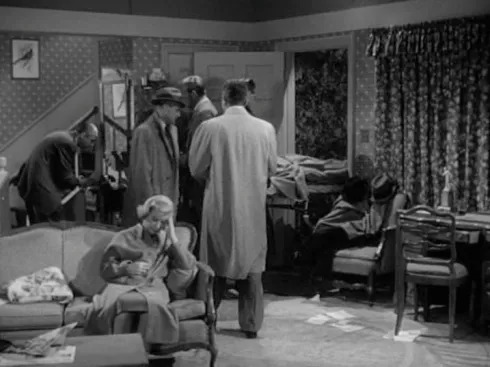
\includegraphics[scale=0.23]{capturfiles_264.jpg}
			\caption[]{The investigation}
		\end{wrapfigure}
		
		\noindent Mr. Maloney was known to be able to extract any data out of any scene, to solve some of the greatest mysteries in Great Britain, and was one of the most honored detectives in the London Police Department. As such, he has had several dangerous opponents--that have come to murder him last night. One of the arrested people, Oliver Jones, was imprisoned for 20 years till last month when the jury found him non-guilty. After the fact, it was found that the jury became one of the wealthiest persons in central London. 
		
		Another theory suggests that Patrick was murdered over fights for the inheritance of his father Oliver Molways, who left approximately half of a million dollars in cash, together with real estate. Since Mr. Molway is known to be close to the jury, he was expected to inherit most of the father's property. 
		
		Mr. Noonan says that ``the police is invastigating the incident, and we have strong avidences condemming Jones as the murder''. When asked about other people that were in the area at the same time, he answered that ``the only known person to be there was Mrs. Maloney, which was validated to be at teh groccer when the murder accured. We're sorry for her loss". 
		
		The funeral will occur next Sunday. His wife and some representatives of the local police station are expected to come. 
		
		Mr. Noonan refused to answer further questions, and seemed confused about the problem. With that said, he was quite sure Oliver Jones would be convicted. Meanwhile, we remain with many questions about what happened to one of the greatest and bravest detectives in Great Britain. 
		
	\end{multicols}
	
	\vfill
	
\end{document}